\label{sec:lifecycle} 
Scientific software is designed to model phenomena in the
physical world. The term 'physical' used here includes chemical and
biological systems since physical processes are underlying building
blocks for those systems too. A phenomenon may be at a microscopic
level, for example protein folding, or at extremely large scales, for
example galaxy cluster mergers.  In some applications multiple scales
are modeled.  The physical characteristics of the systems being
modeled are translated into mathematical models that are said to
describe the essential features of the behavior of the system being 
studied. These equations are then discretized, and numerical algorithms
are used to solve them. One or more parts of this process may
themselves be subjects of active research. Therefore the simulation
software development requires diverse expertise and
adds many stages in the development and lifecycle described below that
may not be encountered elsewhere.  

\subsection{Development Cycle}
\label{sec:dev-cycle}
For scientific simulations, modeling begins with equations that describe the
general class of behavior to be studied, for example, the Navier-Stokes
equations describe the flow of compressible and incompressible
fluids, and van der Waals equations describe interactions among
molecules in a material. There may be more than one set of equations
if all behaviors of interest are not adequately captured by one set.
In translating the model from mathematical representation to
computational representation two processes go on simultaneously,
discretization and approximation. One can argue that discretization is,
by definition, an approximation because it is in effect sampling
continuous behavior where information is lost in the sampling
interval. This loss manifests itself as error terms in the discretized
equations, but error terms are not the only 
approximations. Depending upon the level of understanding of specific
sub-phenomena, and available compute resources, scientists also 
use their judgement to make other approximations. Sometimes, to focus on a
particular behavior, a term in an equation may be simplified or may be even completely
dropped. At other times some physical details may be dropped
from the model because they are not understood well enough by the
scientists.  Or the model itself may be an approximation.  

The next stage in developing the code is finding appropriate
numerical methods for each of the models. Sometimes existing methods 
can be used without modification,  but more often, customization or new
method development is needed. A method's applicability to the model
may need to be validated if the method is new or
significantly modified. Unless a reliable implementation is
already available as a third party software (stand-alone or in a
library), the method has to be implemented and verified. It is at this stage
that the development of a CSE code begins to resemble that of general
software. The numerical algorithms are specified, the semantics are
understood, and they need to be translated into executable
code. Even then there are difference because scientific code
developers work iteratively \cite{segal2005software}, requirement
specifications evolve through the development cycle. 
Figure \ref{Fig:dev-cycle} gives an example of the development
cycle of a multiphysics application modeled using partial differential
equations. 

\begin{figure}[!t]
\centering
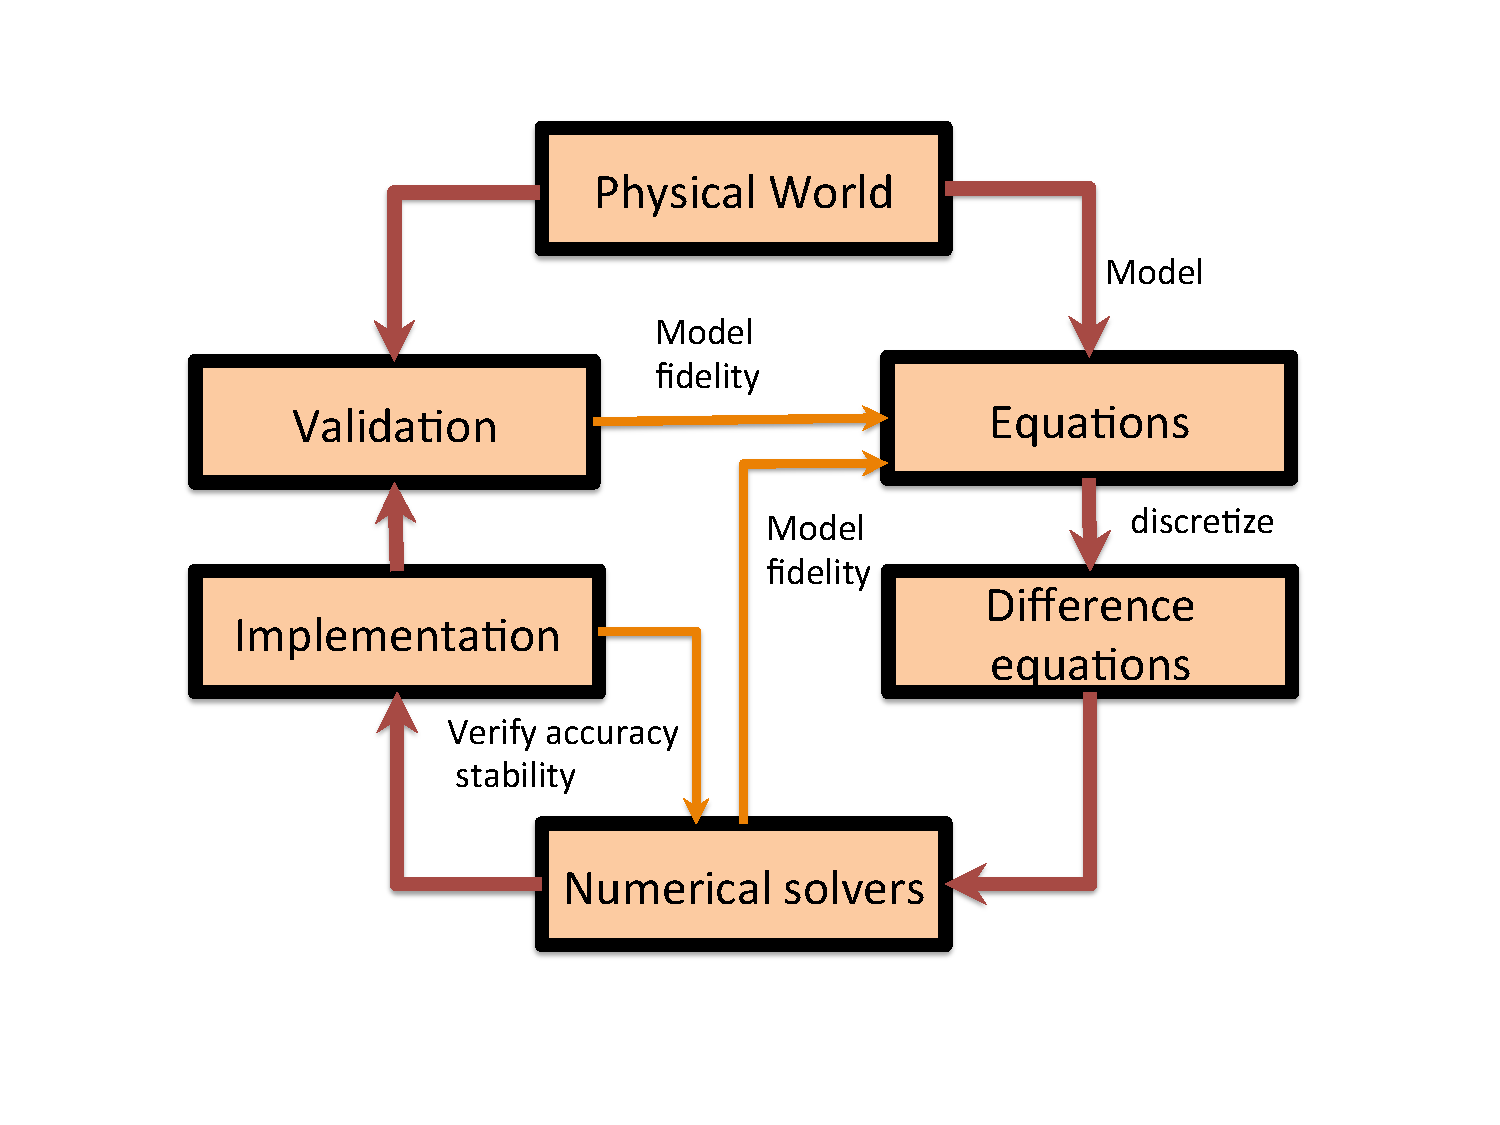
\includegraphics[ width=4.0in]{CSE-design}
\vskip -0.25in
\caption{Development cycle of modeling with partial differential equations}
\label{Fig:dev-cycle}
\end{figure}



\subsection{Verification and Validation}
\label{sec:vandv}
% There are many stages in the development cycle of scientific software 
% where errors can be introduced. 
% Many of the errors introduced in one
% stage have no correlation with those in other stages. A good verification and validation
% methodology will exploit this knowledge .  

The terms verification and validation are often used interchangeably,
but to many scientific domains they have specific meaning.   
In their narrow definition, validation ensures that the mathematical
model correctly defines the physical phenomena, while verification
makes sure that the implementation of the model is correct. In other
words, a model is validated against observations or experiments from
the physical world, whereas a model is verified by other forms of
testing \cite{oberkampf2002verification}.   Other definitions give
broader scope to  verfication and validation (i.e. \cite{sargent1998verification}). For
example, validation of a numerical method may be constructed through
code-to-code comparisons, and its order can be validated through
convergence studies. Similarly, the implementation of a solver can be
validated against an analytically obtained solution for some model if
the same solver can be applied and the analytical solution is also
known, though this is not always possible
\cite{oberkampf2010verification}.  Irrespective of  specific
definitions, what is true is that   correctness must be assured at all
the stages from model to implementation.     

There are many degrees of freedom in the process of deriving a
model as discussed in the previous section, therefore, the validation of the
model must be carefully calibrated by scientific experts. Similarly,
verification of a numerical method requires applied math expertise,
because, in addition to correctness the method needs verification of its stability, accuracy and
order of convergence. Many numerical methods 
%have their own error analysis because of approximations and many of these methods 
are themselves objects of ongoing research, so their
implementation may need modifications from time to time. Whenever
this happens, the entire gamut of verification and validation needs to
be applied again. This is an instance of a particular challenge in 
CSE software where no amount of specification is enough to hand the
implementation over to software engineers or developers who do not
have domain or method knowledge. A close collaboration with applied
mathematicians and method developers is necessary because the process
has to be iterative with scientific judgement applied at every
iteration.  

One other unique verification challenge in CSE software is because of
finite machine precision of floating point numbers. Any change in
compilers, optimization levels, and even order of operations can cause
numerical drift in the solutions
\cite{monniaux2008pitfalls}. Especially in applications that have a
large range of scales, it can be extremely difficult to differentiate
between a legitimate bug and a numerical drift \cite{Dubey2015}. Therefore, relying
upon bitwise reproducibility of the solution is rarely a sufficient
method for verifying the continued correctness of an application
behavior. Robust diagnostics (such as statistics or conservation of
physical quantities) need to be built into the verification process.
This issue is discussed in greater detail in the chapter {\em Testing
  in CSE Software} .  

\subsubsection{Testing}
\label{sec:testing}
%\comment{KA NOTE: KA will expand this section}
Testing of CSE software needs to reflect the layered complexity that
the codes themselves have. The first line of attack is to develop the
unit tests which isolate testing of one component of the
code. However, in CSE codes, often there are dependencies between
different components of the code that can not be meaningfully
isolated, making unit testing more difficult. In these cases, testing
should be done with a minimal possible combination of components.  In
effect, these minimally combined tests play the same role in the
testing regime that unit tests do because they focus on possible
defects in a very narrow section of the code. In addition,
multicomponent CSE software should test various  permutations and
combination of components in different ways. Configuring tests in this
manner will help verify that all configurations are within the
accuracy and stability constraints \cite{Dubey2015}.   

\subsection{Maintenance and Extensions}
\label{sec:maintain}
In a simplified view of software lifecycle, there is a design and development phase,
followed by production and maintenance phase.  Even in well engineered
codes this simplified view typically applies only to the
infrastructure and API's which have a distinct development phase with
limited spill into the remainder of the lifecycle. The numerical 
algorithms and solvers can be in a continually evolving state
reflecting the advances in their respective fields.  
The development of CSE software is usually responding to an immediate
scientific need, so the codes get employed in production as soon as a
minimal set of computational modules necessary for even one scientific
project are built.  Similarly, the development of computational
modules almost never stops all through the code lifecycle because new
findings in science and math almost continuously place new demands on
them. The additions are mostly incremental when they incorporate new
findings into an existing feature, they can also be substantial when
new capabilities are added. The need for new capabilities may arise
from  greater model fidelity, or from trying to simulate a more
complex model. Sometimes a code designed for one scientific field may
have enough in common with another field that capabilities may be
added to enable it for the new field \cite{Dubey2016}.    

Whatever may be the cause, co-existence of development and
production/maintenance phases is a constant challenge to the code
teams. It becomes acute when the code needs to undergo major version
changes. The former can be managed with some repository
discipline in the team coupled with a solid testing regime. The latter
is a much bigger challenge where the plan has to concern itself with
questions such as how much backward compatibility is suitable, how
much code can go offline, and how to reconcile ongoing development in
code sections that are substantially different between versions.
FLASH's example in section \ref{sec:FLASHSoftwareProcess} describes
a couple of strategies that met the conflicting needs of developers and
production users in both scenarios. Both required co-operation and
buy-in from all the stakeholders to be successful. 


\subsection{Performance Portability}
\label{sec:perfport}

%\item performance portability important
%\comment{KA will expand this section}
Another aspect of multiphysics CSE software is its need for
performance portability. HPC machines are expensive and rare resources and in order to achieve high application performance, codes need to be optimized for the unique HPC architectures.
 However, typical lifecycle of a
multiphysics application spans many generations of HPC systems which have a typical lifespan of about 4-5 years.  Depending upon the size of the
code, optimization for a specific target platform can take a
significant fraction of the platform lifecycle, time when the code may not be available for science runs.  Without careful planning and coordination,  a
large fraction of scientists' time could be lost in porting and optimizing
a code for a new system.  Developers have the choice of adding machine
specific optimizations or creating more general optimization that will
work for a broader class of systems.  CSE codes must consider the
trade-offs and advantages of a highly optimized code for a single
platform versus designing their software using constructs that perform
modestly well across a range of platforms. 



\subsection{Using CSE Software}
\label{sec:using}
Users of scientific software must have a basic understanding of the
models, the approximations and the numerical methods they are using to
obtain valid scientific results. They must know and
understand the valid regimes for applicability of numerical
algorithms, as well as their accuracy and stability behavior. For
example a numerical method that can resolve a smooth 
fluid flow only will fail if there are discontinuities. Similarly, in
order to use the Fast Fourier Transform (FFT) method, users must
ensure that their sampling interval resolves all modes. Failure to do
so may filter out important information and lead to wrong results.
Sometimes equations have mathematically valid but physically invalid
solutions. An inappropriately applied numerical scheme may converge to
such a non-physical solution.  

At best any of the above situations lead to a waste of computing resources if the defect in
the solution is detected. At worst they may lead to wrong scientific
conclusions being drawn. Some in the scientific community even argue
that those who have not written at least a simplistic version of the
code for their application should not be using other's code. Though
that argument goes too far, it embodies a general belief in the
scientific community that users of scientific codes have a great
responsibility to know their tools and understand their capabilities
and limitations.  
These are some of the reasons that also play a role in tendency of scientific
codes to do strict gatekeeping for contributions.


